\subsection{Reconhecimento Facial}
\label{subsec:reconhecimento}

	O reconhecimento facial é uma das atividades mais comuns realizadas diariamente
	por seres vivos dotados de certa inteligência. Essa simples atividade vem
	despertando o interesse de pesquisadores que trabalham com computação visual e
	inteligência artificial. O objetivo desses pesquisadores é de construir sistemas
	artificiais capazes de realizar o reconhecimento de faces humanas e a partir
	desta capacidade, construir os mais diferentes tipos de aplicações: sistemas de
	vigilância, controles de acesso, definições automáticas de perfis, entre
	outros~\cite{oliveira}.
	
	No anos 70, os estudos do reconhecimento facial eram baseados sobre atributos
	faciais mensuráveis como olhos, nariz, sobrancelhas, bocas, entre outros. Porém,
	os recursos computacionais eram escassos e os algoritmos de extração de
	características eram ineficientes. Nos anos 90, as pesquisas na área
	ressurgiram, inovando os métodos existentes~\cite{hong, saocarlos} e
	disseminando a técnica.
	
	Umas das maiores dificuldades dos sistemas de reconhecimento é tratar a
	complexidade dos padrões visuais. Mesmo sabendo que todas as faces possuem
	padrões reconhecidos, como boca, olhos e nariz, elas também possuem variações
	únicas que devem ser utilizadas para determinar as características relevantes.
	Outra dificuldade encontrada em relação a essas características é que elas
	possuem uma larga variação estatística para serem consideradas únicas para cada
	indivíduo. O ideal seria que a variância inter-classe seja grande e a
	intra-classe pequena, pois assim imagens de diferentes faces geram os códigos
	mais diferentes possíveis, enquanto imagens de uma mesma face geram os códigos
	mais similares possíveis. Portanto, estabelecer uma representação que capture as
	características ideais é um desafio~\cite{saocarlos}.
	
	Do ponto de vista geral, o reconhecimento facial continua sendo um problema
	aberto por causa de várias dificuldades que aumentam a variância
	intra-classe~\cite{hong}. Entre estas, destacamos as mais
	comuns~\cite{saocarlos}:

	\begin{itemize}
		\item iluminação;
		\item ângulos e poses;
		\item expressões;
		\item cosméticos e acessórios;
		\item extração da face do contexto ou do fundo;
	\end{itemize}

	\begin{figure}[H]
		\begin{center}
			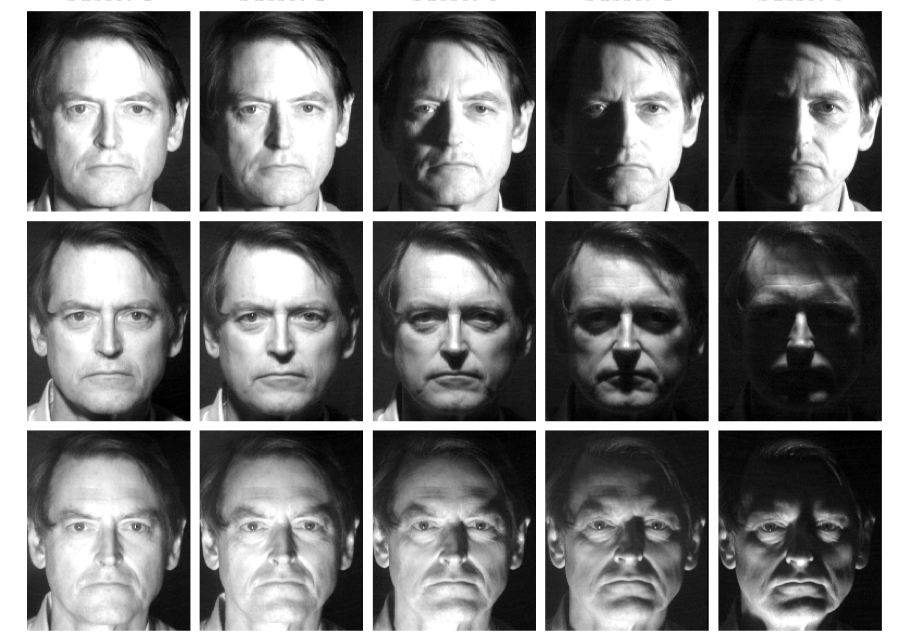
\includegraphics[height=9.5cm,width=12.5cm]{figuras/2.FundamentacaoTeorica/diferencailuminacao.png}
		\end{center}
		\caption{Exemplo de uma imagem de uma pessoa com a mesma expressão facial, vista do mesmo ponto de vista mas sobe diferentes condições de iluminação~\cite{belhumeur}.}
		\label{diferencailuminacao}
	\end{figure}

	Na Figura \ref{diferencailuminacao}, temos um exemplo de como uma mesma pessoa,
	com a mesma expressão facial, vista do mesmo ponto de vista, pode parecer
	drasticamente diferente quando as fontes de luz possuem diferentes
	direções~\cite{belhumeur}.
	
	No contexto de identificação, o reconhecimento facial se resume no
	reconhecimento de um ``retrato'' frontal, estático e controlado. Estático pois
	os ``retratos'' utilizados nada mais são que imagens e controlado pois a iluminação, o fundo, a
	resolução dos dispositivos de aquisição e a distância entre eles e as faces são
	essencialmente fixas durante o processo de aquisição da imagem~\cite{hong}.
	
	Basicamente, o processo de reconhecimento facial pode ser divido em duas tarefas
	principais~\cite{hong}:

	\begin{enumerate}
		\item Detecção de faces em imagens;
		\item Reconhecimento das faces encontradas;
	\end{enumerate}

% ###################################################################################################################

\subsubsection{Detecção de faces em imagens}
\label{ref:viola-jones}
	
	A primeira etapa para o reconhecimento de faces é a detecção de um rosto, e a
	partir daí a comparação do mesmo com modelos conhecidos pelo sistema~\cite{hong,
	oliveira}. Em um sistema de reconhecimento facial, tanto o tempo de resposta
	quanto a confiabilidade desta etapa influenciam diretamente no desempenho e o
	emprego deste sistema~\cite{oliveira}.
	
	A detecção de faces é definida como o processo que determina a existência ou não
	de faces em uma imagem e uma vez encontrada alguma face, sua localização deve
	ser apontada através de um enquadramento ou através de suas coordenadas dentro
	da imagem~\cite{oliveira}. A Figura \ref{enquadramentoRosto} representa um
	exemplo da detecção de uma face em uma imagem.

	\begin{figure}[H]
		\begin{center}
			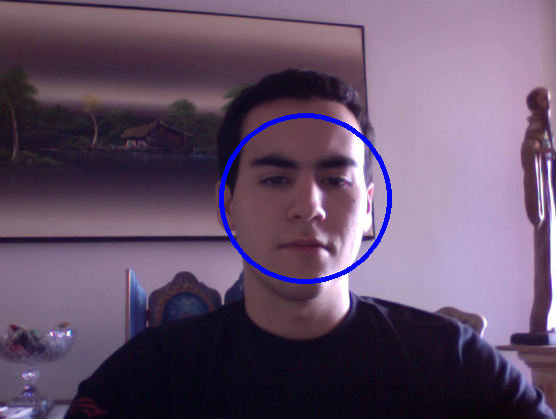
\includegraphics[scale=0.3]{figuras/2.FundamentacaoTeorica/enquadramentoRosto.png}
		\end{center}
		\caption{Exemplo de um processo de detecção de uma face em uma imagem.}
		\label{enquadramentoRosto}
	\end{figure}

	O processo de detecção de faces geralmente é dificultado pelas seguintes razões
	mostradas a seguir:

	\begin{enumerate}
		\item \textbf{Pose}: as imagens de uma face podem variar de acordo com a posição
		relativa entre a câmera e a face (frontal, 45 graus, perfil, ``de cabeça para
		baixo''), e com isso algumas características da face, como olhos e nariz, podem
		ficar parcialmente ou totalmente ocultadas~\cite{yang}.
				 
		\item \textbf{Presença de acessórios}: características faciais básicas
		importantes para o processo de detecção podem ficar ocultadas pela presença de
		acessórios, como óculos, bigode, barba, entre outros~\cite{oliveira, yang}.
		 
		\item \textbf{Expressões faciais}: embora a maioria das faces apresente
		estruturas semelhantes (olhos, bocas, nariz, entre outros) e são dispostas
		aproximadamente na mesma configuração de espaço, pode haver um grande número de
		componentes não rígidos e texturas diferentes entre as faces. Um exemplo são as
		flexibilizações causadas pelas expressões faciais~\cite{oliveira, yang};
				 
		\item \textbf{Obstrução}: faces podem ser obstruídas por outros objetos. Em uma
		imagem com várias faces, uma face pode obstruir outra~\cite{yang}.
		
		\item \textbf{Condições da imagem}: a não previsibilidade das condições da
		imagem em ambientes sem restrições de iluminação, cores e objetos de
		fundo~\cite{oliveira, yang}.
	\end{enumerate}

	Atualmente, já existem diferentes métodos/técnicas de detecção de faces. Tais
	métodos podem ser baseados em imagens de intensidade e em imagens de cor ou
	também em imagens de três dimensões. Os principais métodos de imagens de cor e
	de intensidade podem ser divididos em quatro categorias:

	\begin{enumerate}
		\item \textbf{Métodos baseados em conhecimento:} métodos, desenvolvidos
		principalmente para localização facial, baseados em regras derivadas do
		conhecimento dos pesquisadores do que constitui uma típica face humana.
		Normalmente, captura as relações existentes entre as características faciais. É
		fácil encontrar regras que descrevem as características faciais, por exemplo,
		uma face sempre é constituída por dois olhos simétricos, um nariz e uma boca. As
		relações entre essas características podem ser representadas pelas distâncias
		relativas e posições. Este método possui desvantagens em relação a construção do
		conjunto de regras. Se estas são muito gerais, corre-se o risco, de que o
		sistema que as utilizam, apresentar uma alta taxa de falsos positivos. Se são
		muito específicas, podem ser ineficazes ao tentar detectar faces por não
		satisfazerem todas as regras, diminuindo muito a precisão da
		detecção~\cite{yang,lopes};
		
		\item \textbf{Métodos baseados em características invariantes:} esses algoritmos
		tem como objetivo principal encontrar as características estruturais que existem
		mesmo quando a pose, o ângulo e as condições de iluminação variam. E por meio
		dessas características localizar a face. São desenvolvidos principalmente para
		localização facial~\cite{yang}. A principal desvantagem desse método é que tais
		características invariantes podem ser corrompidas devido a algum tipo de ruído
		ou as fortes variações nas condições de iluminação, comprometendo a eficiência.
		A cor da pele e a textura da face são as principais características invariantes
		que podem ser utilizadas para separar a face de outros objetos~\cite{lopes};
		
		\item \textbf{Métodos baseados em padrões:} vários padrões comuns de um rosto
		são armazenados tanto para descrever o rosto como um todo quanto para descrever
		as características faciais separadamente. As correlações entre as imagens de
		entrada e os padrões armazenados são computados para detecção. Esses métodos são
		desenvolvidos para serem utilizados tanto para localização e como para detecção
		facial~\cite{yang};
		
		\item \textbf{Métodos baseados em aparência:} recebem este nome devido ao fato
		de não utilizarem nenhum conhecimento, a priori, sobre o objeto ou
		características a serem detectadas. Em contraste com os métodos baseado em
		\textit{templates}, os modelos são retirados de um conjunto de imagens de
		treinamento que devem capturar a variabilidade da face. Esses modelos retirados
		são utilizados para detecção. Nesta classe de algoritmos surge os conceitos de
		aprendizado e treinamento, uma vez que as informações necessárias para realizar
		a tarefa de detecção são retiradas do próprio conjunto de imagens sem
		intervenção externa~\cite{yang, lopes}.

	\end{enumerate}

	Um problema relacionado e muito importante é como avaliar a performance dos
	métodos de detecção de faces propostos. Para isso, muitas métricas foram
	adotadas como tempo de aprendizagem, número de amostras necessárias no
	treinamento e a proporção entre taxas de detecção e ``falso alarme''. Esta
	última é dificultada pelas diferentes definições para as taxas de detecção e
	falso alarme adotadas pelos pesquisadores~\cite{yang}.
	
	O método \textit{Viola-Jones} é baseado em padrões para detecção de objetos, o
	que minimiza o tempo de computação, e possui uma alta acurácia permitindo a
	detecção de faces em tempo real. Este método pode ser utilizado para construir
	uma abordagem de detecção facial rápida e eficaz utilizando apenas imagens em
	tons de cinza distinguindo-se dos outros métodos que utilizão informações
	auxiliares como a diferença em sequência de vídeos e o uso de
	cores~\cite{edsonma, violajones}. Apesar da simplicidade obtém altas taxas de
	detecção~\cite{edsonma}. O método é implementado pela biblioteca
	\textit{OpenCV}~\cite{opencv_library} (\textit{Open Source Computer Vision}) e é amplamente utilizado.
	
	O Método \textit{Viola-Jones}~\cite{servodetection,violajones,edsonma} para detecção facial utiliza quatro conceitos
	chaves ilustrados na Figura~\ref{fig:edsonma}:
		
	\begin{enumerate}
		\item \textbf{Características \textit{Haar} básicas:} simples características
		retangulares avaliadas rapidamente por meio de uma nova representação da imagem
		chamada ``Imagem Integral'';
		
		\item \textbf{Imagem Integral:} uma nova representação da imagem que permite uma
		rápida avaliação de recursos e características. Basicamente, o método consiste
		em acrescentar pequenas unidades juntas. Neste caso, pequenas unidades são
		valores de \textit{pixels}. O valor ``integral'' para cada \textit{pixel} é a
		soma de todos os \textit{pixels} acima e a esquerda. Começando pelo canto
		superior esquerdo da imagem e atravessando para direita e para baixo, toda a
		imagem pode ser ``integrada'' com poucas operações por
		\textit{pixel};
		
		\item \textbf{O método \textit{AdaBoost}}: um algoritmo de aprendizado
		\textit{boosting} utilizado para construir um classificador, selecionando um
		pequeno número de características importantes;
		
		\item \textbf{Classificadores em cascata}: classificadores fracos
		\textit{boosted} em uma estrutura de árvore que geram inferências rápidas e
		robustas na construção de um classificador
		forte;
	\end{enumerate}

	\begin{figure}[H]
		\begin{center}
			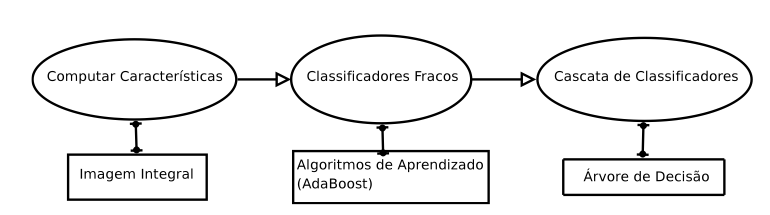
\includegraphics[scale=0.5]{figuras/2.FundamentacaoTeorica/edsonma.png}
		\end{center}
		\caption{Componentes Básicos do Método \textit{Viola-Jones}~\cite{edsonma}.}
		\label{fig:edsonma}
	\end{figure}

	\begin{figure}[H]
		\begin{center}
			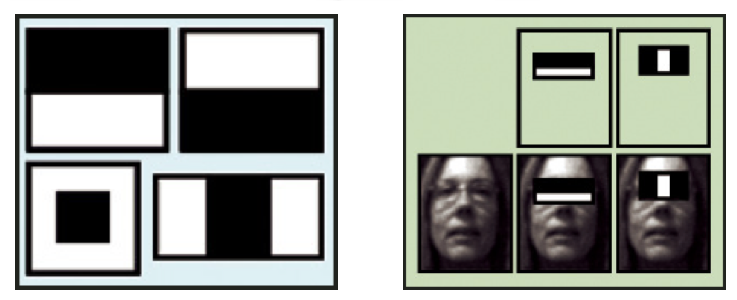
\includegraphics[height=6.5cm,width=12.5cm]{figuras/2.FundamentacaoTeorica/haar_features.png}
		\end{center}
		\caption{Exemplo de Características \textit{Haar} básicas. Adaptada de~\cite{servodetection}.}
		\label{haarfeatures}
	\end{figure}

	A detecção facial em imagens é baseada em simples características retangulares,
	exemplificada na Figura~\ref{haarfeatures}. Existem inúmeros motivos para se
	usar as características retangulares, uma das principais é que sistemas
	baseados em características são muito mais rápidos que sistemas baseados em
	\textit{pixels}~\cite{violajones}.

	\begin{figure}[H]
		\begin{center}
			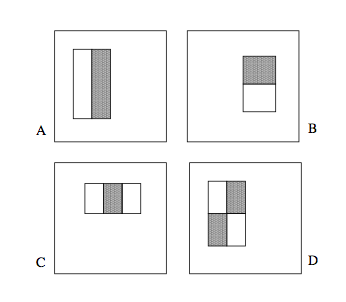
\includegraphics[height=6.5cm,width=12.5cm]{figuras/2.FundamentacaoTeorica/haarfeaturestypes.png}
		\end{center}
		\caption{Características \textit{Haar} básicas com dois, três e quatro retângulos~\cite{violajones}.}
		\label{haarfeaturestypes}
	\end{figure}

	Estas simples características são remanescentes das funções de base
	\textit{Haar}. O método utiliza três tipos de características, exemplificadas na
	Figura \ref{haarfeaturestypes}: características com dois, três ou quatro
	retângulos~\cite{violajones}. A presença de uma característica em uma imagem é
	determinada pela subtração da média dos valores dos \textit{pixels} da região
	escura pela média dos valores dos \textit{pixels} da região clara. Caso o valor
	seja maior que um limiar, então essa característica é tida como
	presente~\cite{servodetection}.

	O método \textit{Viola-Jones} não trabalha diretamente com as intensidades da
	imagem. Para determinar a presença ou ausência de centenas de características
	\textit{Haar} em cada posição de imagem e em várias escalas de forma eficiente,
	utiliza-se uma técnica chamada ``Imagem Integral''~\cite{servodetection,
	violajones}, em que uma nova representação de imagem é criada. Com isso,
	qualquer característica pode ser computada para qualquer escala e localização em
	um tempo constante~\cite{violajones}.

	Para selecionar características \textit{Haar} básicas que serão utilizados e
	para definir os limiares, o método \textit{Viola-Jones} utiliza um método de
	aprendizagem de máquina chamado \textit{AdaBoost}. Este combina vários
	classificadores ``fracos'' para criar um classificador ``forte''.
	
	Um classificador fraco é aquele que só obtém a resposta correta um pouco mais
	frequente que um ``palpite aleatório''. A combinação desses classificadores
	``fracos'', onde cada um ``empurra'' a resposta final um pouco na direção certa,
	pode ser considerado como um classificador ``forte''. O método \textit{AdaBoost}
	seleciona um conjunto de classificadores ``fracos'' para combinar e atribui
	pesos a cada um. Essa combinação ponderada resulta em um classificador
	``forte''~\cite{servodetection}.
	
	Em qualquer região de uma imagem, o número total de características
	\textit{Haar} básicas é muito grande. Para assegurar uma classificação rápida, o
	processo de aprendizagem deve excluir o maior número de características
	disponíveis, e focar nas que são críticas. A seleção dessas características é
	alcançada através de uma simples modificação no método \textit{AdaBoost}: o
	mecanismo de aprendizagem é construído de forma que cada classificador ``fraco''
	retornado dependa de somente uma única característica. Como resultado, cada
	estágio do processo seleciona um novo classificador ``fraco'' o que pode ser
	visto como um processo de seleção de características. O	\textit{AdaBoost}
	fornece um algoritmo de aprendizagem eficaz~\cite{violajones}.

	\begin{figure}[H]
		\begin{center}
			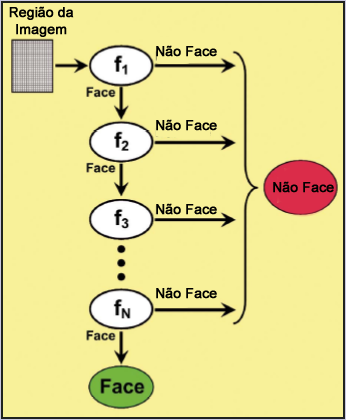
\includegraphics[scale=5.0]{figuras/2.FundamentacaoTeorica/filterchain.png}
		\end{center}
		\caption{Ilustração de uma classificador em cascata composto com uma cadeia de filtros~\cite{servodetection}.}
		\label{filterchain}
	\end{figure}

	O método \textit{Viola-Jones} combina uma série de classificadores
	\textit{AdaBoost} na forma de uma cadeia de filtros, como na Figura
	\ref{filterchain}, que recebe o nome de ``Classificadores em Cascata''. Cada
	filtro em si é um classificador \textit{AdaBoost} com um número relativamente
	pequeno de classificadores ``fracos''~\cite{servodetection}.
	
	O limiar de aceitação, em cada nível, é definido ``baixo'' o suficiente para que
	passe por todos, ou quase todos, os exemplos de face do conjunto de treinamento
	(um grande banco de imagens contendo faces). Os filtros em cada nível são
	treinados para classificar imagens de treinamento que passaram por todas fases
	anteriores~\cite{servodetection}.
	
	Durante a utilização, se alguma região de uma imagem falhar em passar em um
	desses filtros, esta é imediatamente classificada como ``não face''. Quando uma
	região de uma imagem passa por um filtro, ela vai para o próximo filtro na
	cadeia. As regiões das imagens que passarem por todos os filtros na cadeia são
	classificadas como ``faces''~\cite{servodetection}.
	
	O algoritmo utilizado para construção dos ``Classificadores em Cascata'' alcança
	um ótimo desempenho e, ao mesmo tempo, reduz drasticamente o tempo de
	computação. O aspecto chave é que os menores classificadores (filtros), e por
	isso mais eficientes, podem ser utilizados para rejeitar a maioria das regiões
	das imagens que não são faces antes que os classificadores mais complexos sejam
	utilizados~\cite{violajones}. A ordem dos filtros no classificador é baseado nos
	pesos que o método \textit{AdaBoost} define para cada filtro. Os filtros com
	maior peso são colocados no início, para eliminar as regiões das imagens que não
	são faces o mais rápido possível~\cite{servodetection}.
	
	O método \textit{Viola-Jones} é adequado para utilização em sistemas de detecção
	de faces em tempo real. Agora, o próximo passo para o processo de
	``Reconhecimento Facial'' é comparar as faces encontradas com modelos conhecidos
	pelo sistema para realizar a identificação.

% ####################################################################################################################
% ####################################################################################################################
% ####################################################################################################################

\subsubsection{Reconhecimento das Faces encontradas}
\label{sec:reconhecimento}

	Na etapa de reconhecimento, as faces detectadas, serão comparadas com um banco
	de dados de faces conhecidas. Várias técnicas são usadas para acelerar essa
	comparação já que para identificar o usuário é necessário um grande número de
	comparações. Dentre as técnicas utilizadas existem duas variações principais, as
	que usam como entrada dados de imagens de intensidade e de cor e as que usam
	como entradas dados de imagens de profundidade.
	
	As técnicas que utilizam imagens de cor e de intensidade são as mais antigas e
	comuns e são amplamente utilizadas. Dentre elas destacam-se:
	
	\begin{enumerate}
		\item \textbf{\textit{Eigenfaces}:} extrai as informações relevantes de uma
		face, codifica-a da maneira mais eficiente possível, e a compara com um banco de
		faces codificadas de maneira similar. Extrai as informações relevantes contidas
		em uma imagem de uma face de uma maneira simples captando a variação em uma
		coleção de imagens de face e usando essa informação para codificar e comparar
		imagens individuais de faces~\cite{turk}. É baseado em projeção linear das
		imagens em uma espaço de imagens de menor dimensão. Para redução dimensional
		utiliza PCA - ``\textit{Principal Component Analisys} (Análise de componente
		principal)'' maximizando a dispersão total entre todas as
		imagens~\cite{belhumeur};
		
		\item \textbf{Redes Neurais:} uma rede neural artificial é um modelo
		computacional capaz de, entre outras funções, armazenar, classificar padrões,
		realizar interpolação de funções não-lineares e apresentar soluções heurísticas
		para problemas de otimização. Isso é conseguido através de um processo
		denominado ``aprendizado''. O uso de redes neurais visa tornar o sistema de
		reconhecimento capaz de absorver pequenas variações ocorridas no momento da
		coleta de medidas faciais. Espera-se, portanto,  mais robustez a falhas e que
		responda de forma mais confiável~\cite{oliveira};
		
		\item \textbf{\textit{Fisher Faces}:} igual ao \textit{Eigenfaces}, é um método
		que procura uma projeção linear das faces para um espaço dimensional menor onde
		os impactos causados pelas variações de luz e expressões faciais são
		minimizados. O método é derivado da discriminante linear de Fisher
		(FLD)~\cite{belhumeur}.
	\end{enumerate}

	O \textit{Eigenfaces} trata-se de uma técnica bastante satisfatória quando utilizada
	sobre uma base de dados (faces) relativamente grande, permitindo ao sistema
	inferir, das imagens suas principais características e, partindo delas, realizar
	o reconhecimento das imagens utilizando um número bastante reduzido de
	cálculos~\cite{artigo-eigenface}, permitindo, assim, um reconhecimento em tempo
	real.
	
	Os princípios básicos por trás dele, como PCA - ``\textit{Principal Component
	Analisys}'' (Análise de componente principal) e \textit{Distance-Based
	Matching} (Correspondência Baseada na Distância) aparecem cada vez mais na computação
	visual e em diversas aplicações de inteligência artificial~\cite{hewitt}.
	
	Basicamente, as etapas do processo de reconhecimento são simples e bem
	definidas. Dada uma imagem de um rosto desconhecido e imagens do rosto das
	pessoas conhecidas executa as seguintes ações~\cite{hewitt}:

	\begin{enumerate}
		\item Computa a ``distância'' entre a nova imagem e cada uma das imagens já conhecidas.
		\item Seleciona a imagem mais próxima	 do rosto em questão.
		\item Se a ``distância'' da nova imagem para a imagem já catalogada for menor que o limite pré-definido, ``reconhece'' a imagem caso contrário classifica como ``desconhecida''.
	\end{enumerate}

	Em \textit{Eigenfaces}, a distância entre as imagens é medida ponto a ponto
	entre as imagens conhecidas e as desconhecidas. A distância Euclidiana, medida
	entre dois pontos $P_1$ e $P_2$ em duas dimenções, é dada pela fórmula
	$\displaystyle d_{12} = \sqrt{(d_{x} + d_{y})}$, onde $\displaystyle d_x = (x_2
	- x_1)^2$ e $\displaystyle d_y = (y_2-y_1)^2$ e representada na Figura
	\ref{distanciaEntrePontos}~\cite{hewitt}. Para se medir a distância entre as
	imagens usa-se a seguinte formula $\displaystyle d(\vec{X}, \vec{Y}) =
	\sqrt{\sum_{\substack{i=1}}^{n} (x_i-y_i)^2}$~\cite{perlibakas}.

    \begin{figure}[H]
		\begin{center}
			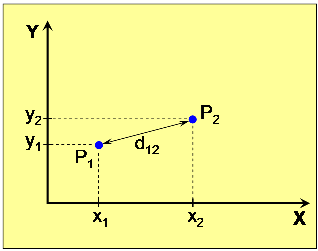
\includegraphics[scale=1.0]{figuras/2.FundamentacaoTeorica/graficoDistanciaEntrePontos.png}
		\end{center}
		\caption{Distância euclidiana entre dois pontos em duas dimensões~\cite{hewitt}.}
		\label{distanciaEntrePontos}
	\end{figure}

	A distância Euclidiana é simples e fácil de implementar mas estudos mostram que
	é possível obter melhores resultados utilizando uma outra distância, conhecida
	como Mahalanobis. Essa distância, usada bastante na estatística, é útil para
	determinar a similaridade de uma amostra desconhecida de uma conhecida. Ao
	contrário da distância Euclidiana, a Mahalanobis correlaciona todos os pontos de
	modo a detectar melhor os padrões existentes. O calculo é feito através da
	formula $\displaystyle d(\vec{X}, \vec{Y}) =  - \frac{1}{\sqrt{\sum_{i=1}^{n}
	x_i^2} \sqrt{\sum_{i=1}^{n} y_i^2}}   \sum_{\substack{i=1}}^{n} z_ix_iy_i$ onde
	$\displaystyle z_i = \sqrt{\frac{\lambda_i}{\lambda_i + \alpha^2}}$ e
	$\displaystyle \alpha = 0,25$~\cite{perlibakas}.
	
	Imagens possuem ``ruídos'' e vamos definir ruído como qualquer coisa que
	atrapalhe na identificação, como por exemplo, as diferenças na luminosidade.
	Cada \textit{pixel} possui uma intensidade de ruído diferente. Com cada
	\textit{pixel} contribuindo para o ruído total, este se torna muito elevado
	comparado com a informação útil que se possa retirar da imagem, dificultando o
	processo de reconhecimento. Uma solução é diminuir a dimensionalidade da imagem,
	tornando assim o ruído menor e possibilitando extrair, da imagem, as informações
	importantes~\cite{hewitt}.
	
	O \textit{Eigenfaces} utiliza o método PCA - ``\textit{Principal Component
	Analisys}'' (Analíse de componente principal) para reduzir a dimensionalidade da
	imagem~\cite{hewitt}. Este método é interessante para dar-nos alguma intuição
	sobre as componentes principais para o nosso conjunto de dados. O lado esquerdo
	da Figura \ref{exemploEigenfaces} mostra as imagens das faces de dez pessoas. O
	lado direito  mostra os seis primeiros componentes principais deste conjunto de
	dados, apresentados como \textit{eigenfaces}. Uma \textit{eigenface} da
	componente principal é uma imagem média de todas as \textit{eigenfaces} que
	estão projetadas na mesma. Essas \textit{eigenfaces} muitas vezes têm um olhar
	fantasmagórico, porque combinam elementos de várias faces. As regiões de
	\textit{pixels} mais brilhantes e as regiões mais escuras em cada imagem são as
	que mais contribuem para as componentes principais~\cite{hewitt}. Cada \textit{eigenface}
	está associada a um \textit{eigenvalue} que representa o quanto as imagens de treinamento
	variam da \textit{eigenface} média naquela direção.
	
	As \textit{eigenfaces} são usadas para que a
	partir delas possa se estimar a distância entre a imagem que se deseja
	reconhecer e as imagens presentes no banco e a partir dessas distâncias dizer de
	qual delas a nova imagem mais se aproxima~\cite{turkpentland}.

	\begin{figure}[H]
		\begin{center}
			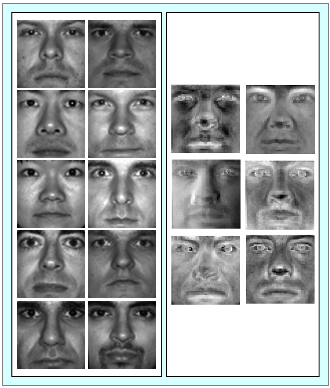
\includegraphics[scale=1.2]{figuras/2.FundamentacaoTeorica/eigenfaces.png}
		\end{center}
		\caption{Direita: imagens de rosto para dez pessoas. Esquerda: os seis primeiros componentes principais, visto como \textit{Eigenfaces}~\cite{hewitt}.}
		\label{exemploEigenfaces}
	\end{figure}

	As componentes principais encontradas pelo PCA apontam para a maior variação de
	dados. Uma das premissas do \textit{Eigenfaces} é que a variabilidade das
	imagens subjacentes corresponde à diferença entre as faces. Esta suposição nem
	sempre é válida. A Figura \ref{exemplosImagensIluminacaoo} mostra as faces de
	dois indivíduos apresentadas em quatro diferentes condições de
	iluminação~\cite{hewitt}. Na verdade, elas são imagens de faces de duas das dez pessoas mostradas na
	Figura \ref{exemploEigenfaces}. Quando a iluminação é muito variável esse
	algoritmo não é muito efetivo~\cite{hewitt}.

	\begin{figure}[H]
		\begin{center}
			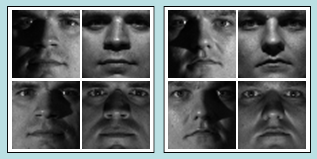
\includegraphics[scale=1.2]{figuras/2.FundamentacaoTeorica/exemplosImagensIluminacaoo.png}
		\end{center}
		\caption{Imagens das faces de dois indivíduos. A face de cada indivíduo é apresentada em quatro diferentes condições de iluminação. A variabilidade devido à iluminação aqui é maior do que a variabilidade entre os indivíduos. \textit{Eigenfaces} tende a confundir as pessoas quando os efeitos de iluminação são muito fortes \cite{hewitt}.}
		\label{exemplosImagensIluminacaoo}
	\end{figure}

	Outros fatores que podem aumentar a variabilidade da imagem em direções que
	tendem a diluir a identidade no espaço PCA incluem mudanças na expressão, ângulo
	da câmera e posição da cabeça~\cite{hewitt}.
	
	A Figura \ref{exemploEspacoPCA} mostra como a distribuição de dados afeta o
	desempenho do \textit{Eigenfaces}. Quando os pontos referentes as imagens de
	cada indivíduo ficam aglutinadas e satisfatoriamente separadas das imagens do conjunto de imagens de outros
	indivíduos temos o melhor caso para o funcionamento do \textit{Eigenfaces}.
	
	Caso os pontos referentes as imagens dos indivíduos tenham uma variabilidade
	muito grande, a probabilidade de choque de imagens de dois indivíduos num mesmo
	ponto do subespaço PCA se torna muito grande tornando extremamente difícil
	separar os dois indivíduos~\cite{hewitt}.
	
	Na prática, a projeção de determinadas imagens de uma pessoa no subespaço PCA
	provavelmente colidirá com projeções de imagens de outras pessoas. Como as \textit{eigenfaces}
	são determinados pela variabilidade dos
	dados, ficamos limitados a quão grande deve ser essa. Podemos tomar medidas para
	limitar, ou para gerir de outra forma, as condições ambientais que podem
	confundi-lo. Por exemplo, colocar a câmera na altura do rosto irá reduzir a
	variabilidade no ângulo da câmera. Porém, alguns fatores são mais difíceis de
	controlar como as condições de iluminação, tais como iluminação lateral vinda de
	uma janela~\cite{hewitt}.
	
	Mesmo com sistemas altamente ajustados, sistemas de reconhecimento facial estão
	sujeitos a casos de identidade equivocada~\cite{hewitt}.

	\begin{figure}[H]
		\begin{center}
			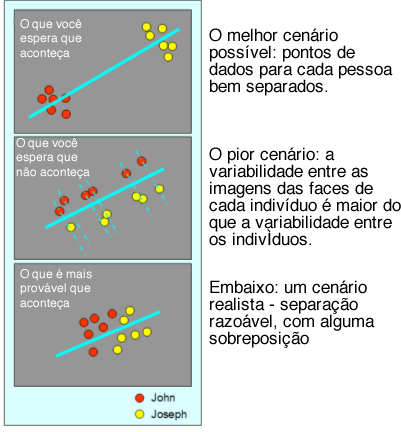
\includegraphics[scale=6.0]{figuras/2.FundamentacaoTeorica/espacoPCA.png}
		\end{center}
		\caption{As distribuições de dados no reconhecimento com \textit{Eigenfaces}. Adapatado de~\cite{hewitt}.}
		\label{exemploEspacoPCA}
	\end{figure}

	Basicamente, a abordagem para o reconhecimento facial com \textit{Eigenfaces} requer as
	seguinte operações de inicialização~\cite{turk}:

	\begin{enumerate}
		\item Adquirir um conjunto inicial de imagens para serem usadas como conjunto inicial de dados;
		\item Treinar o algoritmo calculando a \textit{eigenface} média;
	\end{enumerate}

	Com o sistema inicializado, os seguintes passos devem ser seguidos para
	reconhecer novas imagens de faces~\cite{turk}:
	
	\begin{enumerate}
		\item Projetar a nova imagem na componente principal;
		\item Calcular a distância entre a \textit{eigenface} média e a \textit{eigenface} nova;
		\item Comparar com as distâncias das outras imagens e dizer se é ``conhecida'' ou não de acordo com o limiar de proximidade.
	\end{enumerate}
	
	Após realizar os passos acima, concluindo a detecção e a identificação da face,
	é possível inferir uma label para a imagem com uma determinada confiança.
